\documentclass{beamer}
\usepackage[utf8]{inputenc}
% \usetheme{Copenhagen}
\newcommand{\todo}{\textbf{TODO:} \textbf}
\AtBeginSection[]
{
        \begin{frame}
                \frametitle{Table of Contents}
                \tableofcontents[currentsection]
        \end{frame}
}
\begin{document}
% 20-30

\title{Swiping Burger}
\author{Florian, Steffen, Felix, Lukas}

\frame{\maketitle}

\section{Expose}
\begin{frame}
        \frametitle{Expose}
		\begin{itemize}
		  \item Examination of a sequence of questions in an e-learning app often does not happen sequentially
		  \item Swipe gestures are efficient when going through data sequentially, but how about other scenarios?
		  \item Comparison of Hamburger menu navigation with swipe gestures for large jumps within sequence
		\end{itemize}
\end{frame}

\begin{frame}
        \frametitle{Tasks}
		\begin{itemize}
		  \item Starting at page one, in each task, participant has to visit five pages in a predefined order (kind of a treasure hunt)
		  \item The distances between two pages are once $d - 1$, three times $d$, and once $d + 1$: average distance is $d$
		  \item After completion of a task, questionnaire has to be filled in (built into the application)
		\end{itemize}
\end{frame}

\begin{frame}
        \frametitle{Tasks - Example}


   		\begin{figure}
		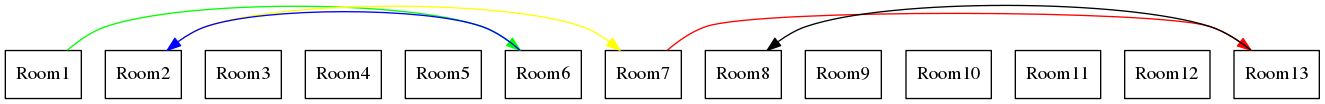
\includegraphics[width=\textwidth]{distance_5.png}
		\caption{A task where $d = 5$}
		\end{figure}
		
		Sequence:
		
		Room1 $\rightarrow$ Room6 $\rightarrow$ Room2 $\rightarrow$ Room7 $\rightarrow$ Room13 $\rightarrow$ Room8

		
\end{frame}

\begin{frame}
  \frametitle{Tasks}
  In total there are five tasks with different distances: 5, 10, 15, 20, 25
  % strategy +d -(d-1) +d +(d+1) -d
  \begin{itemize}
    % 5
    \item Room1 $\rightarrow$ Room6 $\rightarrow$ Room2 $\rightarrow$ Room7 $\rightarrow$ Room13 $\rightarrow$ Room8
      % 10
    \item Room1 $\rightarrow$ Room11 $\rightarrow$ Room2 $\rightarrow$ Room12 $\rightarrow$ Room23 $\rightarrow$ Room13
      % 15
    \item Room1 $\rightarrow$ Room16 $\rightarrow$ Room2 $\rightarrow$ Room17 $\rightarrow$ Room33 $\rightarrow$ Room18
      % 20
    \item Room1 $\rightarrow$ Room21 $\rightarrow$ Room2 $\rightarrow$ Room22 $\rightarrow$ Room43 $\rightarrow$ Room23
      % 25
    \item Room1 $\rightarrow$ Room26 $\rightarrow$ Room2 $\rightarrow$ Room27 $\rightarrow$ Room53 $\rightarrow$ Room28
  \end{itemize}
\end{frame}

\begin{frame}
        \frametitle{Tasks - Realization}
		
		
		\begin{figure}
		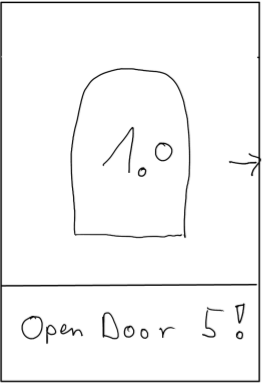
\includegraphics[scale=0.2]{door1_swipe.png}
		\hspace{1cm}
		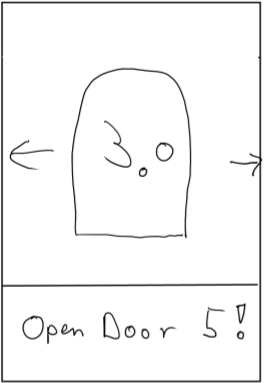
\includegraphics[scale=0.2]{door3_swipe.png}
		\caption{Navigation with swipe gestures}
		\end{figure}
		
		\begin{figure}
		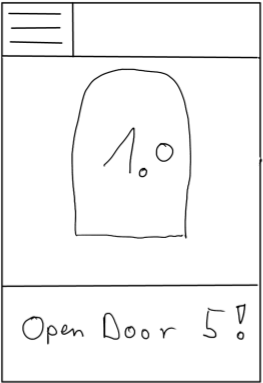
\includegraphics[scale=0.2]{door1_hamburger.png}
		\hspace{1cm}
		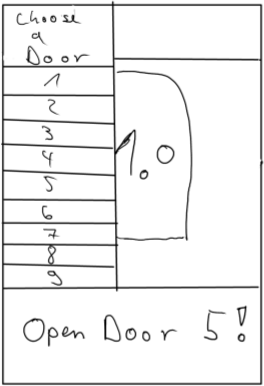
\includegraphics[scale=0.2]{door1_hamburger_open.png}
		\caption{Navigation with Hamburger menu}
		\end{figure}

\end{frame}

\begin{frame}
        \frametitle{Tasks - Realization cont'd}
		
		\begin{figure}
		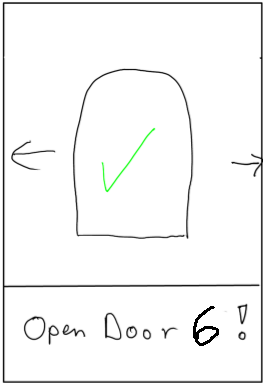
\includegraphics[scale=0.2]{door_opened.png}
		\hspace{1cm}
		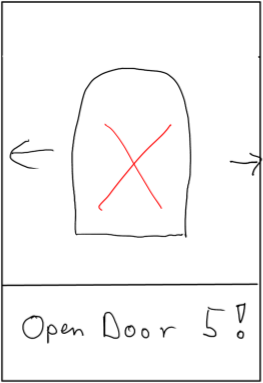
\includegraphics[scale=0.2]{door_opened_failed.png}
		\hspace{1cm}
		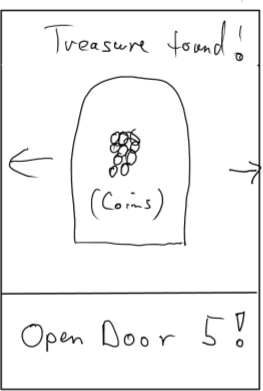
\includegraphics[scale=0.2]{treasure_found.png}
		\caption{Opening the right door, a wrong door, and the last door}
		\end{figure}

\end{frame}

\begin{frame}
        \frametitle{Hypotheses}
        \begin{itemize}
                \item Usage of Hamburger Menu navigation requires constant time to travel a path.
                \item Usage of Swipe navigation
                        results in growing time depending on the distance.
                \item There is some point of intersection,
                        where the required navigation time of Swipe exceeds the required navigation time of Hamburger Menu.
        \end{itemize}

\end{frame}


\section{Design}
\subsection{Within-, Between-group or Split-plot}
\begin{frame}
        \frametitle{Within-, Between-group or Split-plot}
        \begin{itemize}
                \item Between group treatment among navigation methods
                \item Within group design over the length of the navigation paths
        \end{itemize}
        $\rightarrow$ Split-plot design.
\end{frame}

\subsection{Independent and Dependent Variables}
\begin{frame}
        \frametitle{Independent / Dependent Variables}
        \begin{block}{Independent Variables}
                \begin{itemize}
                        \item Navigation Method
                        \item Navigation Distance
                \end{itemize}
        \end{block}
        \begin{block}{Dependent Variables}
                \begin{itemize}
                        \item Time
                        \item User satisfaction (Questionnaires)
                \end{itemize}
        \end{block}
\end{frame}

\subsection{Participants and Location}
\begin{frame}
        \frametitle{Participant Acquisition and where to investigate}
        \begin{block}{Field study}
                \begin{description}
                        \item[Why?] Participants should not get bored.
                                Experiment is not too long.
                        \item[Where?] Mensa: because student's are used to smartphones.
                        \item[When?] Not during meal times to avoid distraction.
                \end{description}
        \end{block}
\end{frame}

\subsection{Questionnaires}
\begin{frame}
        \frametitle{Questionnaires}
        \begin{block}{After each distance block}
                \begin{itemize}
                        \item `` Ich konnte die Aufgaben gut lösen. ''
                        \item `` Die Erreichung des Ziels war mir zu umständlich.''
                \end{itemize}
        \end{block}
        \begin{block}{At the very end}
                \begin{itemize}
                        \item ``Die Umgebung hat mich beim Bearbeiten der Aufgaben gestört''
                        \item ``Die Dauer des Experiments war mir zu hoch?''
                        \item ``Die Bedienung des mobilen Geräts war intuitiv''
                        \item ``Die Art der Navigation hat mir zugesagt''
                \end{itemize}
        \end{block}
\end{frame}

\section{Analysis Methods}
\begin{frame}
  \frametitle{Main Idea}
  \begin{itemize}
    \item \textbf{Given}:
      Required time, for each navigation method (swipe, burger) and for each
      distance $d \in D$.
    \item \textbf{Wanted}: Point of intersection, distance  $d^*$, at which Swipe
      navigation becomes less efficient than Hamburger Menu navigation.
    \item \textbf{The Plan}:
      \begin{enumerate}
        \item Compare the different distances \emph{within} one navigation
          method to each other.
        \item Draw a comparison \emph{between} the two
          navigation methods.
      \end{enumerate}
  \end{itemize}
\end{frame}

\begin{frame}
  \frametitle{Hamburger Menu Navigation over distances $D$}
  \begin{itemize}
    \item Consider normally distributed random variables $X_d$ with means $\bar x_d$
      and variance $\sigma_{x}^2$ being the time required for traveling
      $d$ pages using Hamburger Menu navigation.
    \item We hypothesize that
      \begin{align*}
        H_0^\text{burger}: \bar x_{d_1} = \bar x_{d_2} = \cdots = \bar x_{d_{|D|}}
      \end{align*}
    \item Since we can assume equal variances, we evaluate the hypothesis using
      Repeated Measures {ANOVA}.
    \item In case we do not find significant differences, we can use the overall mean
      $\bar x$ for comparison with the Swipe navigation.
  \end{itemize}
\end{frame}

\begin{frame}
  \frametitle{Swipe Menu Navigation over distances $D$}
  \begin{itemize}
    \item  Consider normally
      distributed random variables $Y_d$ with means $\bar y_d$ and variances
      $\sigma_{y,d}^2$ being the time required for traveling $d$ pages using
      Swipe navigation.
    \item Then we assert that the following hypothesis can be rejected:
      \begin{align*}
        H_0^\text{swipe}: \bar y_{d_1} = \bar y_{d_2} = \cdots = \bar y_{d_{|D|}}
      \end{align*}
      Since we can not assume homogeneity of variance in this case,
      we evaluate the hypothesis using the Friedmann test.
  \end{itemize}
\end{frame}

\begin{frame}
  \frametitle{Swipe Navigation vs Hamburger Menu Navigation}
  \begin{itemize}
    \item In case we can reject $H_0^\text{swipe}$ and can not reject $H_0^\text{burger}$:
    \item Compare per-distance means $\bar y_d$ of Swipe navigation
      with overall mean $\bar x$ of Hamburger Menu navigation:
      \begin{align*}
        H_0^{(d)} : \bar y_d = \bar x \;\forall d \in D
      \end{align*}
    \item We evaluate these hypotheses using the Welch's $t$-test, because we
      can not assume equal variances.
    \item In the end, we (hopefully) find the distance $d^*$, for which the
      required time with Swipe navigation exceeds the required time with
      Hamburger Menu navigation.
  \end{itemize}
\end{frame}

\section{Discussion}
\begin{frame}
  \frametitle{Discussion}
  \begin{itemize}
    \item Where would you expect the point of intersection $d^*$ to be?
  \end{itemize}
\end{frame}
\end{document}
